% Options for packages loaded elsewhere
% Options for packages loaded elsewhere
\PassOptionsToPackage{unicode}{hyperref}
\PassOptionsToPackage{hyphens}{url}
\PassOptionsToPackage{dvipsnames,svgnames,x11names}{xcolor}
%
\documentclass[
  spanish,
  letterpaper,
  DIV=11,
  numbers=noendperiod,
  oneside]{scrartcl}
\usepackage{xcolor}
\usepackage[left=1in,marginparwidth=2.0666666666667in,textwidth=4.1333333333333in,marginparsep=0.3in]{geometry}
\usepackage{amsmath,amssymb}
\setcounter{secnumdepth}{-\maxdimen} % remove section numbering
\usepackage{iftex}
\ifPDFTeX
  \usepackage[T1]{fontenc}
  \usepackage[utf8]{inputenc}
  \usepackage{textcomp} % provide euro and other symbols
\else % if luatex or xetex
  \usepackage{unicode-math} % this also loads fontspec
  \defaultfontfeatures{Scale=MatchLowercase}
  \defaultfontfeatures[\rmfamily]{Ligatures=TeX,Scale=1}
\fi
\usepackage{lmodern}
\ifPDFTeX\else
  % xetex/luatex font selection
\fi
% Use upquote if available, for straight quotes in verbatim environments
\IfFileExists{upquote.sty}{\usepackage{upquote}}{}
\IfFileExists{microtype.sty}{% use microtype if available
  \usepackage[]{microtype}
  \UseMicrotypeSet[protrusion]{basicmath} % disable protrusion for tt fonts
}{}
\makeatletter
\@ifundefined{KOMAClassName}{% if non-KOMA class
  \IfFileExists{parskip.sty}{%
    \usepackage{parskip}
  }{% else
    \setlength{\parindent}{0pt}
    \setlength{\parskip}{6pt plus 2pt minus 1pt}}
}{% if KOMA class
  \KOMAoptions{parskip=half}}
\makeatother
% Make \paragraph and \subparagraph free-standing
\makeatletter
\ifx\paragraph\undefined\else
  \let\oldparagraph\paragraph
  \renewcommand{\paragraph}{
    \@ifstar
      \xxxParagraphStar
      \xxxParagraphNoStar
  }
  \newcommand{\xxxParagraphStar}[1]{\oldparagraph*{#1}\mbox{}}
  \newcommand{\xxxParagraphNoStar}[1]{\oldparagraph{#1}\mbox{}}
\fi
\ifx\subparagraph\undefined\else
  \let\oldsubparagraph\subparagraph
  \renewcommand{\subparagraph}{
    \@ifstar
      \xxxSubParagraphStar
      \xxxSubParagraphNoStar
  }
  \newcommand{\xxxSubParagraphStar}[1]{\oldsubparagraph*{#1}\mbox{}}
  \newcommand{\xxxSubParagraphNoStar}[1]{\oldsubparagraph{#1}\mbox{}}
\fi
\makeatother


\usepackage{longtable,booktabs,array}
\usepackage{calc} % for calculating minipage widths
% Correct order of tables after \paragraph or \subparagraph
\usepackage{etoolbox}
\makeatletter
\patchcmd\longtable{\par}{\if@noskipsec\mbox{}\fi\par}{}{}
\makeatother
% Allow footnotes in longtable head/foot
\IfFileExists{footnotehyper.sty}{\usepackage{footnotehyper}}{\usepackage{footnote}}
\makesavenoteenv{longtable}
\usepackage{graphicx}
\makeatletter
\newsavebox\pandoc@box
\newcommand*\pandocbounded[1]{% scales image to fit in text height/width
  \sbox\pandoc@box{#1}%
  \Gscale@div\@tempa{\textheight}{\dimexpr\ht\pandoc@box+\dp\pandoc@box\relax}%
  \Gscale@div\@tempb{\linewidth}{\wd\pandoc@box}%
  \ifdim\@tempb\p@<\@tempa\p@\let\@tempa\@tempb\fi% select the smaller of both
  \ifdim\@tempa\p@<\p@\scalebox{\@tempa}{\usebox\pandoc@box}%
  \else\usebox{\pandoc@box}%
  \fi%
}
% Set default figure placement to htbp
\def\fps@figure{htbp}
\makeatother


% definitions for citeproc citations
\NewDocumentCommand\citeproctext{}{}
\NewDocumentCommand\citeproc{mm}{%
  \begingroup\def\citeproctext{#2}\cite{#1}\endgroup}
\makeatletter
 % allow citations to break across lines
 \let\@cite@ofmt\@firstofone
 % avoid brackets around text for \cite:
 \def\@biblabel#1{}
 \def\@cite#1#2{{#1\if@tempswa , #2\fi}}
\makeatother
\newlength{\cslhangindent}
\setlength{\cslhangindent}{1.5em}
\newlength{\csllabelwidth}
\setlength{\csllabelwidth}{3em}
\newenvironment{CSLReferences}[2] % #1 hanging-indent, #2 entry-spacing
 {\begin{list}{}{%
  \setlength{\itemindent}{0pt}
  \setlength{\leftmargin}{0pt}
  \setlength{\parsep}{0pt}
  % turn on hanging indent if param 1 is 1
  \ifodd #1
   \setlength{\leftmargin}{\cslhangindent}
   \setlength{\itemindent}{-1\cslhangindent}
  \fi
  % set entry spacing
  \setlength{\itemsep}{#2\baselineskip}}}
 {\end{list}}
\usepackage{calc}
\newcommand{\CSLBlock}[1]{\hfill\break\parbox[t]{\linewidth}{\strut\ignorespaces#1\strut}}
\newcommand{\CSLLeftMargin}[1]{\parbox[t]{\csllabelwidth}{\strut#1\strut}}
\newcommand{\CSLRightInline}[1]{\parbox[t]{\linewidth - \csllabelwidth}{\strut#1\strut}}
\newcommand{\CSLIndent}[1]{\hspace{\cslhangindent}#1}

\ifLuaTeX
\usepackage[bidi=basic]{babel}
\else
\usepackage[bidi=default]{babel}
\fi
% get rid of language-specific shorthands (see #6817):
\let\LanguageShortHands\languageshorthands
\def\languageshorthands#1{}


\setlength{\emergencystretch}{3em} % prevent overfull lines

\providecommand{\tightlist}{%
  \setlength{\itemsep}{0pt}\setlength{\parskip}{0pt}}



 


\usepackage{booktabs}
\usepackage{longtable}
\usepackage{array}
\usepackage{multirow}
\usepackage{wrapfig}
\usepackage{float}
\usepackage{colortbl}
\usepackage{pdflscape}
\usepackage{tabu}
\usepackage{threeparttable}
\usepackage{threeparttablex}
\usepackage[normalem]{ulem}
\usepackage{makecell}
\usepackage{xcolor}
\KOMAoption{captions}{tableheading}
\makeatletter
\@ifpackageloaded{caption}{}{\usepackage{caption}}
\AtBeginDocument{%
\ifdefined\contentsname
  \renewcommand*\contentsname{Tabla de contenidos}
\else
  \newcommand\contentsname{Tabla de contenidos}
\fi
\ifdefined\listfigurename
  \renewcommand*\listfigurename{Listado de Figuras}
\else
  \newcommand\listfigurename{Listado de Figuras}
\fi
\ifdefined\listtablename
  \renewcommand*\listtablename{Listado de Tablas}
\else
  \newcommand\listtablename{Listado de Tablas}
\fi
\ifdefined\figurename
  \renewcommand*\figurename{Figura}
\else
  \newcommand\figurename{Figura}
\fi
\ifdefined\tablename
  \renewcommand*\tablename{Tabla}
\else
  \newcommand\tablename{Tabla}
\fi
}
\@ifpackageloaded{float}{}{\usepackage{float}}
\floatstyle{ruled}
\@ifundefined{c@chapter}{\newfloat{codelisting}{h}{lop}}{\newfloat{codelisting}{h}{lop}[chapter]}
\floatname{codelisting}{Listado}
\newcommand*\listoflistings{\listof{codelisting}{Listado de Listados}}
\makeatother
\makeatletter
\makeatother
\makeatletter
\@ifpackageloaded{caption}{}{\usepackage{caption}}
\@ifpackageloaded{subcaption}{}{\usepackage{subcaption}}
\makeatother
\makeatletter
\@ifpackageloaded{sidenotes}{}{\usepackage{sidenotes}}
\@ifpackageloaded{marginnote}{}{\usepackage{marginnote}}
\makeatother
\usepackage{bookmark}
\IfFileExists{xurl.sty}{\usepackage{xurl}}{} % add URL line breaks if available
\urlstyle{same}
\hypersetup{
  pdflang={es},
  colorlinks=true,
  linkcolor={blue},
  filecolor={Maroon},
  citecolor={Blue},
  urlcolor={Blue},
  pdfcreator={LaTeX via pandoc}}


\author{}
\date{}
\begin{document}


\pandocbounded{
\includegraphics[keepaspectratio]{images/logo_isuc.png}}

\pandocbounded{
\includegraphics[keepaspectratio]{images/jusmer_trans.png}}

\section{\texorpdfstring{\textbf{Preferencias por la
comodificación}}{Preferencias por la comodificación}}\label{preferencias-por-la-comodificaciuxf3n}

\subsection{\texorpdfstring{\textbf{El rol de la movilidad social
intergeneracional y las creencias meritocráticas en
Chile}}{El rol de la movilidad social intergeneracional y las creencias meritocráticas en Chile}}\label{el-rol-de-la-movilidad-social-intergeneracional-y-las-creencias-meritocruxe1ticas-en-chile}

\begin{center}\rule{0.5\linewidth}{0.5pt}\end{center}

\textbf{Andreas Laffert\textsuperscript{1,2}}

\textbf{\textsuperscript{1}Instituto de Sociología, Pontificia
Universidad Católica de Chile}

\textbf{\textsuperscript{2}Centro de Estudios de Conflicto y Cohesión
Social - COES}

Coloquio de Investigación en Justicia Distributiva y Desigualdad
Socioeconómica

4 Septiembre 2025, Santiago

\begin{center}\rule{0.5\linewidth}{0.5pt}\end{center}

\subsection{¿A dónde quiero llegar?}\label{a-duxf3nde-quiero-llegar}

\section{Contexto y motivación}\label{contexto-y-motivaciuxf3n}

\subsection{Contexto y motivación}\label{contexto-y-motivaciuxf3n-1}

\subsection{Antecedentes}\label{antecedentes}

\begin{enumerate}
\def\labelenumi{\arabic{enumi})}
\tightlist
\item
  Privatización y mercantilización de bienes públicos, políticas de
  bienestar y servicios sociales (Gingrich, 2011; Streeck, 2016)
\end{enumerate}

\begin{enumerate}
\def\labelenumi{\arabic{enumi})}
\setcounter{enumi}{1}
\tightlist
\item
  En AL y Chile, modificaron la arquitectura de las instituciones del
  bienestar expandiendo lógica de mercado (Ferre, 2023; Madariaga, 2020)
\end{enumerate}

\begin{enumerate}
\def\labelenumi{\arabic{enumi})}
\setcounter{enumi}{2}
\tightlist
\item
  Este orden económico se refleja en una economía moral específica (Mau,
  2015; Svallfors, 2006)
\end{enumerate}

Preferencias por justicia de mercado (Busemeyer, 2014; Castillo et~al.,
2025; Immergut \& Schneider, 2020; Koos \& Sachweh, 2019; Lindh, 2015)

\subsection{Preferencias por justicia de
mercado}\label{preferencias-por-justicia-de-mercado}

\begin{itemize}
\item
  Lane (1986): justicia de mercado vs.~justicia política
\item
  Creencias normativas que legitiman la idea de que el acceso a los
  servicios sociales esenciales ---como la salud, la educación o las
  pensiones--- debe determinarse según criterios basados en el mercado
  (Lindh, 2015, p. 895)
\item
  Medición: evaluar si las personas consideran justo que el acceso a
  dichos servicios dependa de los ingresos (Castillo et~al., 2025;
  Kluegel et~al., 1999; Lindh, 2015)
\end{itemize}

Preferencias por la comodificación de servicios

\subsection{Preferencias por justicia de
mercado}\label{preferencias-por-justicia-de-mercado-1}

\subsubsection{Contextual}\label{contextual}

\begin{itemize}
\tightlist
\item
  Gasto social (Busemeyer, 2014; Busemeyer \& Iversen, 2020; Immergut \&
  Schneider, 2020)
\item
  Desigualdad económica (Koos \& Sachweh, 2019)
\item
  Nivel de privatización de servicios y regulación del mercado (Koos \&
  Sachweh, 2019; Lindh, 2015)
\end{itemize}

\subsubsection{Individual}\label{individual}

\begin{itemize}
\tightlist
\item
  Estatus socioeconómico -ingresos, educación y ocupación- (Busemeyer \&
  Iversen, 2020; Koos \& Sachweh, 2019; Lindh, 2015; Svallfors, 2007)
\item
  Percepciones sobre la desigualdad y meritocracia (Castillo et~al.,
  2025)
\item
  Conservadurismo/liberalismo económico (Lee \& Stacey, 2023)
\end{itemize}

\subsection{Preferencias por justicia de mercado:
Chile}\label{preferencias-por-justicia-de-mercado-chile}

\begin{enumerate}
\def\labelenumi{\arabic{enumi}.}
\item
  Otero \& Mendoza (2024) proveen evidencia sobre:

  \begin{itemize}
  \tightlist
  \item
    Personas en posiciones sociales bajas/subordinadas muestran menor
    apoyo a la justicia de mercado que aquellas en posiciones
    altas/privilegiadas.
  \end{itemize}
\item
  Castillo et~al. (2025) encuentran que:

  \begin{itemize}
  \tightlist
  \item
    La percepción de la desigualdad económica reduce el apoyo a la
    justicia de mercado.
  \item
    Las percepciones meritocráticas (esfuerzo) aumenta el respaldo a la
    justicia de mercado.
  \end{itemize}
\end{enumerate}

\subsection{Este estudio}\label{este-estudio}

Cómo la movilidad social afecta estas preferencias sigue sin respuesta

El movimiento entre posiciones expone experiencias y \textbf{mecanismos}
que afectan nociones de justicia

\section{}\label{section}

\textbf{\emph{(1) ¿Cómo la movilidad social intergeneracional afecta las
preferencias por comodificación en salud, pensiones y educación en
Chile?}}

\textbf{\emph{(2) ¿Cómo las creencias meritocráticas median esta
relación en el contexto chileno?}}

\subsection{Movilidad social}\label{movilidad-social}

\subsubsection{Afecta}\label{afecta}

\begin{itemize}
\tightlist
\item
  Preferencias redistributivas (Alesina et~al., 2018; Ares, 2020; Breen
  \& Ermisch, 2024; Schmidt, 2011)
\item
  Creencias sobre la desigualdad (Bucca, 2016; Day \& Fiske, 2017;
  Gugushvili, 2016b; Shariff et~al., 2016)
\item
  Apoyo al gasto social y políticas de bienestar (Gugushvili, 2016a,
  2017)
\end{itemize}

\subsubsection{Mecanismos}\label{mecanismos}

\begin{itemize}
\tightlist
\item
  Intereses materiales (Helgason \& Rehm, 2025)
\item
  Socialización (Jaime-Castillo \& Marqués-Perales, 2019)
\item
  \textbf{Self-serving bias} (Gugushvili, 2016a; Molina et~al., 2019;
  Schmidt, 2011).
\item
  Meritocracia como proxy al sesgo de atribuciones internas y externas
  (Young, 1958)
\end{itemize}

\subsection{Contexto chileno}\label{contexto-chileno}

\begin{itemize}
\tightlist
\item
  Crecimiento con elevada desigualdad (Flores et~al., 2020; Llorca-Jaña
  \& Miller, 2021)
\item
  Profunda privatización y comodificación de áreas de reproducción
  social con fuerte dependencia Estatal (Boccardo, 2020; Madariaga,
  2020)
\item
  Rigida movilidad relativa y fuerte clausura cúspide (López-Roldán \&
  Fachelli, 2021; Torche, 2014)
\item
  Conflictividad social (Núcleo de Sociología Contingente, 2020; Somma
  et~al., 2021) y legitimidad de la desigualdad (Canales Cerón et~al.,
  2021; Castillo et~al., 2025; Panes, 2020)
\end{itemize}

\subsection{Hipótesis}\label{hipuxf3tesis}

\section{Método}\label{muxe9todo}

\subsection{Estrategia de identificación
causal}\label{estrategia-de-identificaciuxf3n-causal}

\subsection{Datos}\label{datos}

\begin{itemize}
\item
  Encuesta Longitudinal Social de Chile
  \href{https://coes.cl/elsoc/}{(ELSOC)} de COES.
\item
  Muestra analítica: olas 2016 (N = 2.927), 2018 (N = 3.748) y 2023 (N =
  2.726)
\item
  Encuesta panel representativa de zonas urbanas, localizadas en 40
  ciudades del país (92 comunas y 13 regiones)
\item
  Diseño muestral complejo: probabilístico, por conglomerados,
  multietápico y estratificado según el tamaño de las ciudades.
\item
  Población objetivo incluye a mujeres y hombres de entre 18 y 75 años
  que residen habitualmente en viviendas privadas
\end{itemize}

\subsection{Outcome}\label{outcome}

\subsection{Tratamiento}\label{tratamiento}

Siguiendo la propuesta de Breen \& Ermisch (2024) para estimar el efecto
causal de la movilidad social:

\begin{enumerate}
\def\labelenumi{\arabic{enumi}.}
\item
  \textbf{Asignación de clase}: En base a la ocupación (ISCO-08) del
  padre/madre y del entrevistado se crean estratos de origen y destino
  (bajo, medio y alto) según terciles de la distribución del índice de
  estatus ocupacional (ISEI)
\item
  \textbf{Propensity-score estimation}: Se estima la probabilidad de
  movilidad social mediante un modelo logístico multinomial en relación
  con las trayectorias inmóviles para cada estrato (categ. ref.). Estas
  puntuaciones de propensión se emplean posteriormente para ajustar la
  selección en la movilidad al evaluar su efecto.
\end{enumerate}

\subsection{Tratamiento}\label{tratamiento-1}

\begin{table}

\caption{\label{tbl-ocup}Movilidad ocupacional por grupos ocupacionales}

\centering{

}

\end{table}%

\begin{itemize}
\tightlist
\item
  \emph{N} (id único) = 4.447. Porcentajes en azul corresponde a las
  filas y en verde a las columnas.
\end{itemize}

\subsection{Tratamiento}\label{tratamiento-2}

\subsection{Mediador}\label{mediador}

\begin{itemize}
\item
  \textbf{Meritocracia}: se mide a partir de dos componentes, a saber,
  el esfuerzo y el talento (Young, 1958)
\item
  Medición:

  \begin{itemize}
  \tightlist
  \item
    Ítem esfuerzo: ``En Chile, se recompensa a las personas por su
    esfuerzo''
  \item
    Ítem talento: ``En Chile, se recompensa a las personas por su
    inteligencia y habilidades''
  \item
    Ambos ítems se responden en una escala Likert de 1 (totalmente en
    desacuerdo) a 5 (totalmente de acuerdo)
  \end{itemize}
\end{itemize}

\subsection{Estimand y estimando}\label{estimand-y-estimando}

\begin{itemize}
\tightlist
\item
  Métodos
\end{itemize}

\section{Resultados}\label{resultados}

\subsection{Modelos}\label{modelos}

\begin{figure}

\caption{\label{fig-mh}Estimaciones de efectos de mobilidad en
preferencia por comodificación en salud}

\centering{

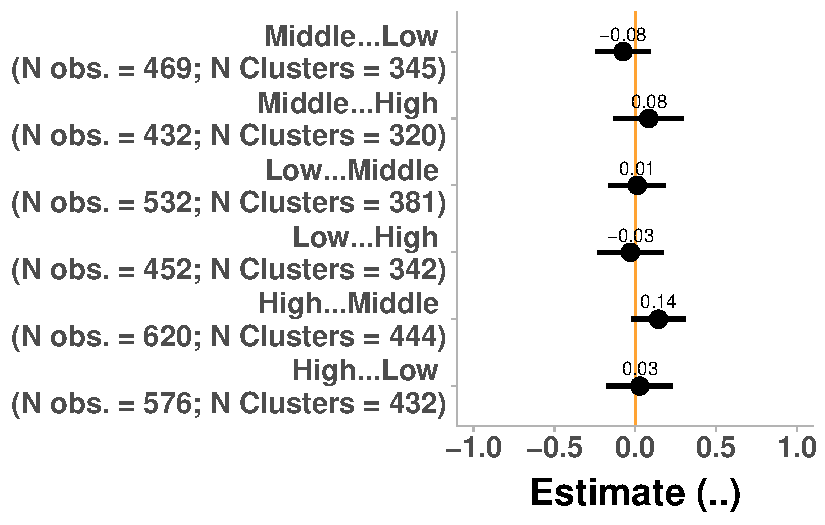
\includegraphics[width=1.8\linewidth,height=\textheight,keepaspectratio]{mjp-mobility_files/figure-pdf/fig-mh-1.pdf}

}

\end{figure}%

\subsection{Modelos}\label{modelos-1}

\begin{figure}

\caption{\label{fig-me}Estimaciones de efectos de mobilidad en
preferencia por comodificación en educación}

\centering{

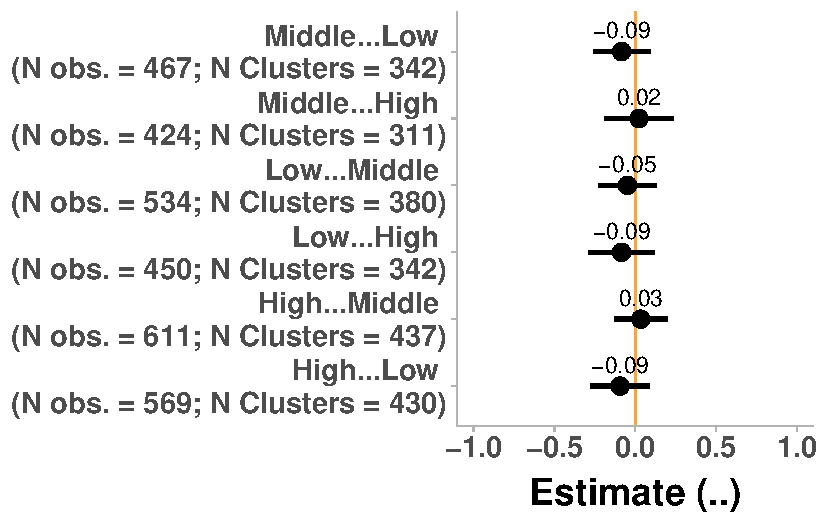
\includegraphics[width=1.8\linewidth,height=\textheight,keepaspectratio]{mjp-mobility_files/figure-pdf/fig-me-1.pdf}

}

\end{figure}%

\subsection{Modelos}\label{modelos-2}

\begin{figure}

\caption{\label{fig-mp}Estimaciones de efectos de mobilidad en
preferencia por comodificación en pensiones}

\centering{

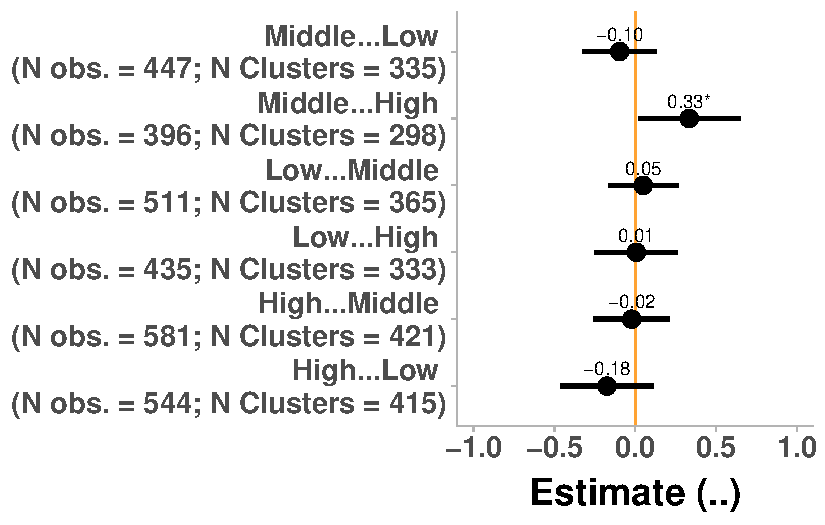
\includegraphics[width=1.8\linewidth,height=\textheight,keepaspectratio]{mjp-mobility_files/figure-pdf/fig-mp-1.pdf}

}

\end{figure}%

\section{Discusión y proyecciones}\label{discusiuxf3n-y-proyecciones}

\section{Discusión y proyecciones}\label{discusiuxf3n-y-proyecciones-1}

\begin{enumerate}
\def\labelenumi{\arabic{enumi}.}
\tightlist
\item
  \textbf{Movilidad social}: ascendente (Middle→High) \emph{incrementa}
  la preferencia por comodificación en pensiones (dominio), no en otros.
\item
  \textbf{Contexto chileno}: profunda comodificación y privatización de
  servicios escenciales → trabajador-empresario
\item
  \textbf{Mediación}: rol de la meritocracia como mediador → ACME (Imai
  et~al., 2010), moderación (?)
\end{enumerate}

\section{Gracias por su atención!}\label{gracias-por-su-atenciuxf3n}

\begin{itemize}
\tightlist
\item
  \textbf{Github del proyecto:}
  \url{https://github.com/Andreas-Lafferte/mobility-market-justice}
\end{itemize}

\subsection*{Referencias}\label{referencias}
\addcontentsline{toc}{subsection}{Referencias}

\phantomsection\label{refs}
\begin{CSLReferences}{1}{0}
\bibitem[\citeproctext]{ref-alesina_intergenerational_2018}
Alesina, A., Stantcheva, S., \& Teso, E. (2018). Intergenerational
{Mobility} and {Preferences} for {Redistribution}. \emph{American
Economic Review}, \emph{108}(2), 521-554.
\url{https://doi.org/10.1257/aer.20162015}

\bibitem[\citeproctext]{ref-ares_changing_2020}
Ares, M. (2020). Changing Classes, Changing Preferences: How Social
Class Mobility Affects Economic Preferences. \emph{West European
Politics}, \emph{43}(6), 1211-1237.
\url{https://doi.org/10.1080/01402382.2019.1644575}

\bibitem[\citeproctext]{ref-boccardo_30_2020}
Boccardo, G. (2020). \emph{30 A{ñ}os de Privatizaciones En {Chile}: Lo
Que La Pandemia Revel{ó}} (Nodo XXI). Santiago.

\bibitem[\citeproctext]{ref-breen_effects_2024}
Breen, R., \& Ermisch, J. (2024). The {Effects} of {Social Mobility}.
\emph{Sociological Science}, \emph{11}, 467-488.
\url{https://doi.org/10.15195/v11.a17}

\bibitem[\citeproctext]{ref-bucca_merit_2016}
Bucca, M. (2016). Merit and Blame in Unequal Societies: {Explaining
Latin Americans}' Beliefs about Wealth and Poverty. \emph{Research in
Social Stratification and Mobility}, \emph{44}, 98-112.
\url{https://doi.org/10.1016/j.rssm.2016.02.005}

\bibitem[\citeproctext]{ref-busemeyer_skills_2014}
Busemeyer, M. (2014). \emph{Skills and {Inequality}: {Partisan Politics}
and the {Political Economy} of {Education Reforms} in {Western Welfare
States}}. Cambridge University Press.

\bibitem[\citeproctext]{ref-busemeyer_welfare_2020}
Busemeyer, M., \& Iversen, T. (2020). The {Welfare State} with {Private
Alternatives}: {The Transformation} of {Popular Support} for {Social
Insurance}. \emph{The Journal of Politics}, \emph{82}(2), 671-686.
\url{https://doi.org/10.1086/706980}

\bibitem[\citeproctext]{ref-canalesceron_sujeto_2021}
Canales Cerón, M., Orellana Calderón, V. S., \& Guajardo Mañán, F.
(2021). Sujeto y Cotidiano En La Era Neoliberal: El Caso de La
Educaci{ó}n Chilena. \emph{Revista Mexicana de Ciencias Pol{í}ticas y
Sociales}, \emph{67}(244).
\url{https://doi.org/10.22201/fcpys.2448492xe.2022.244.70386}

\bibitem[\citeproctext]{ref-castillo_perceptions_2025}
Castillo, J. C., Laffert, A., Carrasco, K., \& Iturra, J. (2025).
Perceptions of {Inequality} and {Meritocracy}: {Their Interplay} in
{Shaping Preferences} for {Market Justice} in {Chile} (2016-2023).
\emph{Under Review at Frontiers in Sociology}.

\bibitem[\citeproctext]{ref-day_movin_2017}
Day, M. V., \& Fiske, S. T. (2017). Movin' on {Up}? {How Perceptions} of
{Social Mobility Affect Our Willingness} to {Defend} the {System}.
\emph{Social Psychological and Personality Science}, \emph{8}(3),
267-274. \url{https://doi.org/10.1177/1948550616678454}

\bibitem[\citeproctext]{ref-ferre_welfare_2023}
Ferre, J. C. (2023). Welfare Regimes in Twenty-First-Century {Latin
America}. \emph{Journal of International and Comparative Social Policy},
\emph{39}(2), 101-127. \url{https://doi.org/10.1017/ics.2023.16}

\bibitem[\citeproctext]{ref-flores_top_2020}
Flores, I., Sanhueza, C., Atria, J., \& Mayer, R. (2020). Top {Incomes}
in {Chile}: {A Historical Perspective} on {Income Inequality},
1964--2017. \emph{Review of Income and Wealth}, \emph{66}(4), 850-874.
\url{https://doi.org/10.1111/roiw.12441}

\bibitem[\citeproctext]{ref-gingrich_making_2011}
Gingrich, J. R. (2011). \emph{Making {Markets} in the {Welfare State}:
{The Politics} of {Varying Market Reforms}} (1.ª ed.). Cambridge
University Press. \url{https://doi.org/10.1017/CBO9780511791529}

\bibitem[\citeproctext]{ref-gugushvili_intergenerational_2016c}
Gugushvili, A. (2016a). Intergenerational Objective and Subjective
Mobility and Attitudes towards Income Differences: Evidence from
Transition Societies. \emph{Journal of International and Comparative
Social Policy}, \emph{32}(3), 199-219.
\url{https://doi.org/10.1080/21699763.2016.1206482}

\bibitem[\citeproctext]{ref-gugushvili_intergenerational_2016}
Gugushvili, A. (2016b). Intergenerational {Social Mobility} and {Popular
Explanations} of {Poverty}: {A Comparative Perspective}. \emph{Social
Justice Research}, \emph{29}(4), 402-428.
\url{https://doi.org/10.1007/s11211-016-0275-9}

\bibitem[\citeproctext]{ref-gugushvili_subjective_2017}
Gugushvili, A. (2017). Subjective {Intergenerational Mobility} and
{Support} for {Welfare State Programmes}.

\bibitem[\citeproctext]{ref-helgason_class_2025}
Helgason, A. F., \& Rehm, P. (2025). Class Experiences and the Long-Term
Evolution of Economic Values. \emph{Social Forces}, \emph{103}(3),
1125-1143. \url{https://doi.org/10.1093/sf/soae135}

\bibitem[\citeproctext]{ref-imai_identification_2010}
Imai, K., Keele, L., \& Yamamoto, T. (2010). Identification, {Inference}
and {Sensitivity Analysis} for {Causal Mediation Effects}.
\emph{Statistical Science}, \emph{25}(1).
\url{https://doi.org/10.1214/10-STS321}

\bibitem[\citeproctext]{ref-immergut_it_2020}
Immergut, E. M., \& Schneider, S. M. (2020). Is It Unfair for the
Affluent to Be Able to Purchase {«Better»} Healthcare? {Existential}
Standards and Institutional Norms in Healthcare Attitudes across 28
Countries. \emph{Social Science \& Medicine}, \emph{267}, 113146.
\url{https://doi.org/10.1016/j.socscimed.2020.113146}

\bibitem[\citeproctext]{ref-jaime-castillo_social_2019}
Jaime-Castillo, A. M., \& Marqués-Perales, I. (2019). Social Mobility
and Demand for Redistribution in {Europe}: A Comparative Analysis.
\emph{The British Journal of Sociology}, \emph{70}(1), 138-165.
\url{https://doi.org/10.1111/1468-4446.12363}

\bibitem[\citeproctext]{ref-kluegel_legitimation_1999}
Kluegel, J. R., Mason, D. S., \& Wegener, B. (1999). The {Legitimation}
of {Capitalism} in the {Postcommunist Transition}: {Public Opinion}
about {Market Justice}, 1991-1996. \emph{European Sociological Review},
\emph{15}(3), 251-283. Recuperado de
\url{https://www.jstor.org/stable/522731}

\bibitem[\citeproctext]{ref-koos_moral_2019}
Koos, S., \& Sachweh, P. (2019). The Moral Economies of Market
Societies: Popular Attitudes towards Market Competition, Redistribution
and Reciprocity in Comparative Perspective. \emph{Socio-Economic
Review}, \emph{17}(4), 793-821. \url{https://doi.org/10.1093/ser/mwx045}

\bibitem[\citeproctext]{ref-lane_market_1986}
Lane, R. E. (1986). Market {Justice}, {Political Justice}.
\emph{American Political Science Review}, \emph{80}(2), 383-402.
\url{https://doi.org/10.2307/1958264}

\bibitem[\citeproctext]{ref-lee_fairness_2023}
Lee, J.-S., \& Stacey, M. (2023). Fairness Perceptions of Educational
Inequality: The Effects of Self-Interest and Neoliberal Orientations.
\emph{The Australian Educational Researcher}.
\url{https://doi.org/10.1007/s13384-023-00636-6}

\bibitem[\citeproctext]{ref-lindh_public_2015}
Lindh, A. (2015). Public {Opinion} against {Markets}? {Attitudes}
towards {Market Distribution} of {Social Services} -- {A Comparison} of
17 {Countries}. \emph{Social Policy \& Administration}, \emph{49}(7),
887-910. \url{https://doi.org/10.1111/spol.12105}

\bibitem[\citeproctext]{ref-llorca-jana_historia_2021}
Llorca-Jaña, M., \& Miller, R. M. D. (2021). \emph{{Historia econ{ó}mica
de Chile desde la independencia}}. Santiago de Chile: RIL editores.

\bibitem[\citeproctext]{ref-lopez-roldan_comparative_2021}
López-Roldán, P., \& Fachelli, S. (Eds.). (2021). \emph{Towards a
{Comparative Analysis} of {Social Inequalities} between {Europe} and
{Latin America}}. Cham: Springer International Publishing.
\url{https://doi.org/10.1007/978-3-030-48442-2}

\bibitem[\citeproctext]{ref-madariaga_three_2020}
Madariaga, A. (2020). The Three Pillars of Neoliberalism: {Chile}'s
Economic Policy Trajectory in Comparative Perspective.
\emph{Contemporary Politics}, \emph{26}(3), 308-329.
\url{https://doi.org/10.1080/13569775.2020.1735021}

\bibitem[\citeproctext]{ref-mau_inequality_2015}
Mau, S. (2015). \emph{Inequality, {Marketization} and the {Majority
Class}: {Why Did} the {European Middle Classes Accept Neo-Liberalism}?}
Houndmills: Palgrave Macmillan.

\bibitem[\citeproctext]{ref-molina_its_2019}
Molina, M. D., Bucca, M., \& Macy, M. W. (2019). It's Not Just How the
Game Is Played, It's Whether You Win or Lose. \emph{SCIENCE ADVANCES}.

\bibitem[\citeproctext]{ref-nucleodesociologiacontingente_informe_2020}
Núcleo de Sociología Contingente, {[}NUDESOC{]}. (2020). \emph{Informe
de Resultados Oficial {Encuesta Zona Cero}}. Santiago de Chile.

\bibitem[\citeproctext]{ref-otero_power_2024}
Otero, G., \& Mendoza, M. (2024). The {Power} of {Diversity}: {Class},
{Networks} and {Attitudes Towards Inequality}. \emph{Sociology},
\emph{58}(4), 851-876. \url{https://doi.org/10.1177/00380385231217625}

\bibitem[\citeproctext]{ref-panes_criticas_2020}
Panes, D. (2020). \emph{Cr{í}ticas y Experiencias Obreras En Torno al
Sistema de {AFP}'s En {Chile} (1981-2020)} (Tesis doctoral). Universidad
de Chile, Santiago.

\bibitem[\citeproctext]{ref-schmidt_experience_2011}
Schmidt, A. W. (2011). The Experience of Social Mobility and the
Formation of Attitudes toward Redistribution. En.

\bibitem[\citeproctext]{ref-shariff_income_2016}
Shariff, A. F., Wiwad, D., \& Aknin, L. B. (2016). Income {Mobility
Breeds Tolerance} for {Income Inequality}: {Cross-National} and
{Experimental Evidence}. \emph{Perspectives on Psychological Science},
\emph{11}(3), 373-380. \url{https://doi.org/10.1177/1745691616635596}

\bibitem[\citeproctext]{ref-somma_no_2021}
Somma, N. M., Bargsted, M., Disi Pavlic, R., \& Medel, R. M. (2021). No
Water in the Oasis: The {Chilean Spring} of 2019--2020. \emph{Social
Movement Studies}, \emph{20}(4), 495-502.
\url{https://doi.org/10.1080/14742837.2020.1727737}

\bibitem[\citeproctext]{ref-streeck_how_2016}
Streeck, W. (2016). \emph{How Will Capitalism End? Essays on a Failing
System}. London: Verso.

\bibitem[\citeproctext]{ref-svallforsMoralEconomyClass2006a}
Svallfors, S. (2006). \emph{The {Moral Economy} of {Class}: {Class} and
{Attitudes} in {Comparative Perspective}}. Stanford University Press.

\bibitem[\citeproctext]{ref-svallfors_political_2007}
Svallfors, S. (Ed.). (2007). \emph{The {Political Sociology} of the
{Welfare State}: {Institutions}, {Social Cleavages}, and {Orientations}}
(1.ª ed.). Stanford University Press.
\url{https://doi.org/10.2307/j.ctvr0qv0q}

\bibitem[\citeproctext]{ref-torche_intergenerational_2014}
Torche, F. (2014). Intergenerational {Mobility} and {Inequality}: {The
Latin American Case}. \emph{Annual Review of Sociology}, \emph{40}(1),
619-642. \url{https://doi.org/10.1146/annurev-soc-071811-145521}

\bibitem[\citeproctext]{ref-young_rise_1958}
Young, M. (1958). \emph{The Rise of the Meritocracy}. New Brunswick,
N.J., U.S.A: Transaction Publishers.

\end{CSLReferences}




\end{document}
